% This LaTeX was auto-generated from MATLAB code.
% To make changes, update the MATLAB code and export to LaTeX again.

\documentclass{article}

\usepackage[utf8]{inputenc}
\usepackage[T1]{fontenc}
\usepackage{lmodern}
\usepackage{graphicx}
\usepackage{color}
\usepackage{hyperref}
\usepackage{amsmath}
\usepackage{amsfonts}
\usepackage{epstopdf}
\usepackage[table]{xcolor}
\usepackage{matlab}

\sloppy
\epstopdfsetup{outdir=./}
\graphicspath{ {./example7_2_images/} }

\begin{document}

\matlabtitle{k-Means algorithm example (Example 7.1)}

\begin{par}
\begin{flushleft}
Introduce the data
\end{flushleft}
\end{par}

\begin{matlabcode}
X1 = [2,10];
X2 = [2,5];
X3 = [8,4];
X4 = [5,8];
X5 = [7,5];
X6 = [6,4];
X7 = [1,2];
X8 = [4,9];

D = [X1;X2;X3;X4;X5;X6;X7;X8];
z = zeros([8,1]);
D = [D,z]
\end{matlabcode}
\begin{matlaboutput}
D = 8x3    
     2    10     0
     2     5     0
     8     4     0
     5     8     0
     7     5     0
     6     4     0
     1     2     0
     4     9     0

\end{matlaboutput}
\begin{matlabcode}
Y = [X5; X6; X8]
\end{matlabcode}
\begin{matlaboutput}
Y = 3x2    
     7     5
     6     4
     4     9

\end{matlaboutput}

\begin{par}
\begin{flushleft}
Apply k-Medians
\end{flushleft}
\end{par}

\begin{matlabcode}
%First iteration
[D,Ynext] = kMediansIter(D,Y,3);
%Plot
c1 = D(:,3) == 1;
c2 = D(:,3) == 2;
c3 = D(:,3) == 3;
scatter(D(c1,1),D(c1,2), 'MarkerFaceColor', 'b');
hold on
scatter(Y(1,1),Y(1,2), 'MarkerFaceColor', 'b');
scatter(D(c2,1),D(c2,2), 'MarkerFaceColor', 'g');
scatter(Y(2,1),Y(2,2), 'MarkerFaceColor', 'g');
scatter(D(c3,1),D(c3,2), 'MarkerFaceColor', 'r');
scatter(Y(3,1),Y(3,2), 'MarkerFaceColor', 'r');
hold off
\end{matlabcode}
\begin{center}
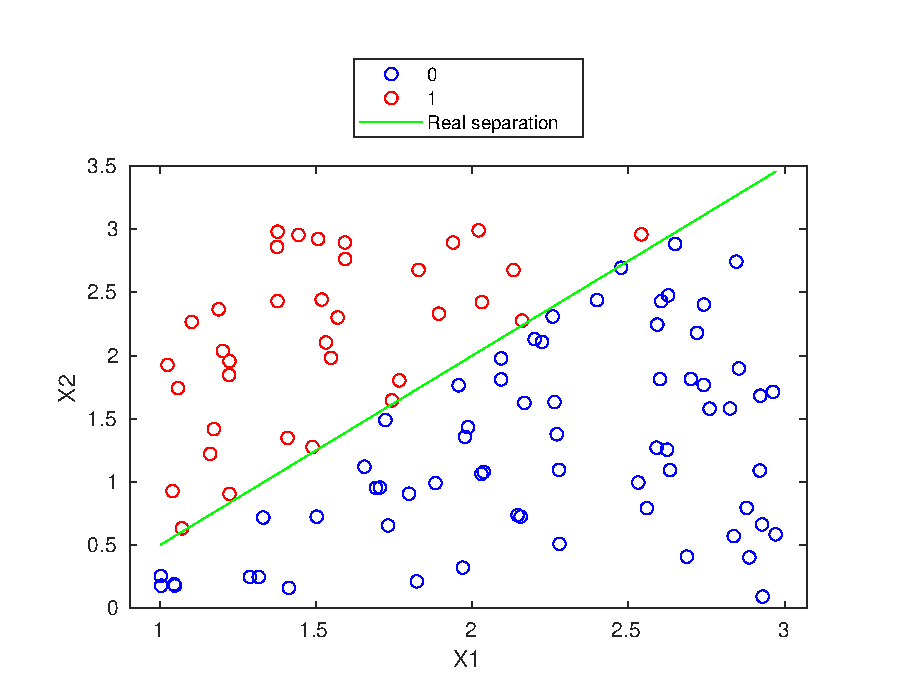
\includegraphics[width=\maxwidth{56.69844455594581em}]{figure_0.eps}
\end{center}
\begin{matlabcode}
Y = Ynext;

%Second iteration
%First iteration
[D,Ynext] = kMediansIter(D,Y,3);
%Plot
c1 = D(:,3) == 1;
c2 = D(:,3) == 2;
c3 = D(:,3) == 3;
scatter(D(c1,1),D(c1,2), 'MarkerFaceColor', 'b');
hold on
scatter(Y(1,1),Y(1,2), 'MarkerFaceColor', 'b');
scatter(D(c2,1),D(c2,2), 'MarkerFaceColor', 'g');
scatter(Y(2,1),Y(2,2), 'MarkerFaceColor', 'g');
scatter(D(c3,1),D(c3,2), 'MarkerFaceColor', 'r');
scatter(Y(3,1),Y(3,2), 'MarkerFaceColor', 'r');
hold off
\end{matlabcode}
\begin{center}
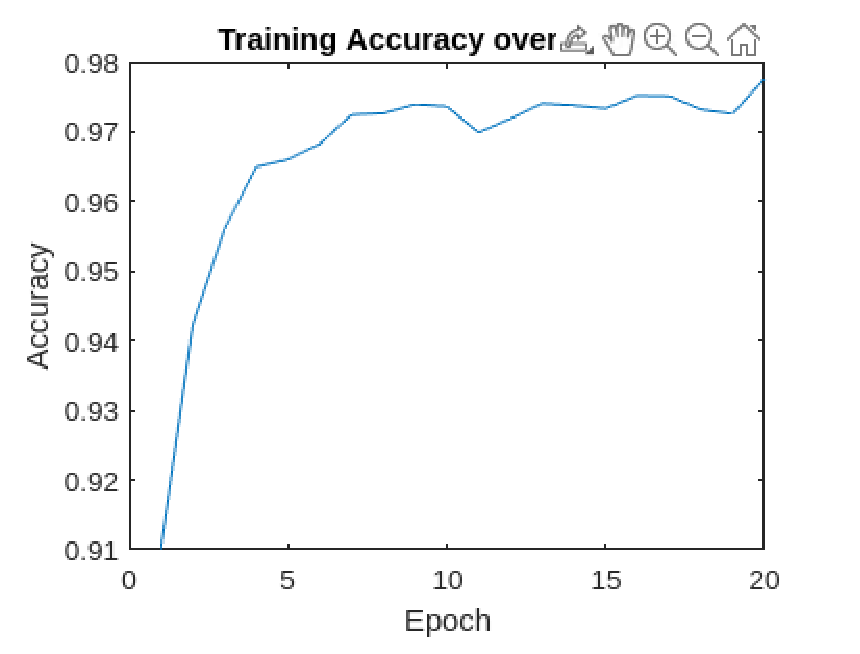
\includegraphics[width=\maxwidth{56.69844455594581em}]{figure_1.eps}
\end{center}
\begin{matlabcode}
Y = Ynext;

%Third iteration
[D,Ynext] = kMediansIter(D,Y,3);
%Plot
c1 = D(:,3) == 1;
c2 = D(:,3) == 2;
c3 = D(:,3) == 3;
scatter(D(c1,1),D(c1,2), 'MarkerFaceColor', 'b');
hold on
scatter(Y(1,1),Y(1,2), 'MarkerFaceColor', 'b');
scatter(D(c2,1),D(c2,2), 'MarkerFaceColor', 'g');
scatter(Y(2,1),Y(2,2), 'MarkerFaceColor', 'g');
scatter(D(c3,1),D(c3,2), 'MarkerFaceColor', 'r');
scatter(Y(3,1),Y(3,2), 'MarkerFaceColor', 'r');
hold off
\end{matlabcode}
\begin{center}
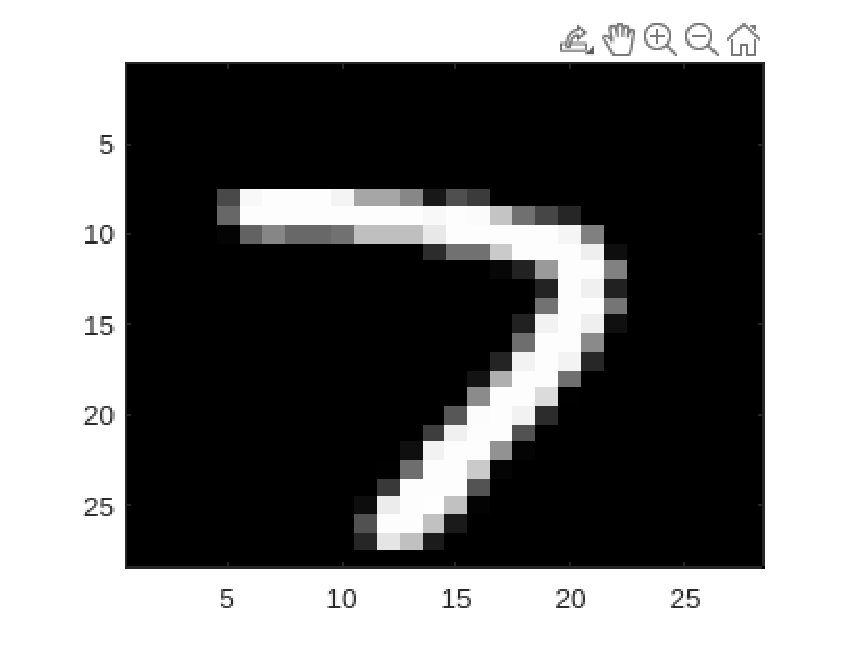
\includegraphics[width=\maxwidth{56.69844455594581em}]{figure_2.eps}
\end{center}
\begin{matlabcode}
Y = Ynext;
\end{matlabcode}


\begin{matlabcode}
function d = distance(X, Y, m)
    n = length(X);
    d = 0;
    for i=1:n
        d = d + abs(X(i)-Y(i))^m;
    end
    d = sqrt(d);
end

function [D2,Ynext] = kMediansIter(D,Y,k)
    dist = zeros(k);
    [n,m] = size(D);
    %Distances
    for j=1:k
        for i=1:n
            dist(i,j)=distance(D(i,1:2),Y(j,:),2);
        end
    end
    %Assign
    [v, idx] = min(dist, [], 2);
    D2 = D;
    D2(:,3) = idx;
    %Optimize
    Ynext = Y;
    for i=1:3
        ci = D2(:,3) == i;
        x = median(D(ci,1));
        y = median(D(ci,2));
        Ynext(i,:)=[x,y];
    end
end
\end{matlabcode}

\end{document}
